\documentclass[letter,12pt]{article}

\usepackage{amssymb}%*
\usepackage{amsthm}
\usepackage{amsfonts}%*
\usepackage[latin2]{inputenc}%*
\usepackage{amsmath}%*
\usepackage{anysize}%*
\usepackage{hyperref}
\usepackage{bbm}
\usepackage{float}
\usepackage{graphicx}
%\usepackage{titlesec}
%\titleformat{\section}
%  {\normalfont\large\bfseries}
%  {\thesection}{1em}{}
%\titleformat{\subsection}
%  {\normalfont\bfseries}
%  {\thesubsection}{1em}{}
\marginsize{2.6cm}{2.6cm}{1cm}{2cm}

\newtheorem*{theorem*}{Theorem}
\newtheorem{main_theorem}{Theorem}
\newtheorem{theorem}{Theorem}[section]

\newtheorem{hint}[main_theorem]{Hint}
\newtheorem*{hint*}{Hint}

\newtheorem{problem}[main_theorem]{Problem}
\newtheorem{extraproblem}[main_theorem]{Extra Proplem}

\newtheorem{main_lemma}[main_theorem]{Lemma}
\newtheorem{main_corollary}[main_theorem]{Corollary}
\newtheorem{main_remark}[main_theorem]{Remark}

\newtheorem{lemma}[theorem]{Lemma}
\newtheorem{corollary}[theorem]{Corollary}
\newtheorem{remark}[theorem]{Remark}
\newtheorem{example}[theorem]{Example}
\newtheorem{definition}[theorem]{Definition}
\newtheorem{proposition}[theorem]{Proposition}

\newcommand{\answerspacetop}{
	\begin{center}
		\textbf{BEGIN YOUR ANSWER BELOW THIS LINE} \\ \hrulefill
	\end{center}
}

\graphicspath{{./}{./images/}}

\title{MATH430 Spring 2024 Homework 1 \\ \normalsize{Due Feb. 5 in online}}
\date{\small{Please write-up your solutions to problems in an organized fashion. Write each problem on a separate sheet. \textbf{Argue each step of your solution.} Every problem is worth 10 points. Partial credit is possible if clear progress is made towards solving the problem. Collaboration is encouraged, but assignment needs to be submitted individually.
If collaborating, please write the names of the people with whom you collaborated next to each solution to help the grader. If a solution is typed in Latex you get 20\% extra credit. Following the provided hints is optional.}}
\begin{document}
\maketitle


\begin{problem} Using a straightedge and compass, construct the following:
\begin{enumerate}
\item Given a segment $[AB]$, construct points $C$,  $C'$, $C''$  such that $m(\widehat{CAB}) = 30^o$, $m(\widehat{C'AB}) = 15^o$ and $m(\widehat{C''AB}) = 45^o$.
    \item Given a segment of a unit length, construct a segment of length $\sqrt[4]{2}$.
\end{enumerate}
\end{problem}
\textbf{Warning:} Please do not just draw pictures; argue each of your solution steps!

\answerspacetop
1. 
Make a circle that take segment $[AB]$ as diameter. The mid point is $O$.
\begin{center}
	\begin{tabular}{c}
		\includegraphics[width=0.7\columnwidth]{Q1A_1.png} \\
	\end{tabular}
\end{center}

Because the line is crossing $O$ and perpendicular to $[AB]$, the intersection of line and circle is $C''$ and thus $AO$ = $C''O$, creating isosceles right triangle $AOC''$. 
\begin{center}
	\begin{tabular}{c}
		\includegraphics[width=0.5\columnwidth]{Q1A_2.png} \\
	\end{tabular}
\end{center}

Make a circle with radius same as $OB$, set the center at $B$. The intersection of the circle(center $B$) and circle(center $O$) will be $C$. This will give us a right triangle (Select any point on the circle and connect this point to the two ends of the diameter to form a right triangle) with ratio of the base to the chord length is $1:2$. Thus $\angle CAB = 30^o$.
\begin{center}
	\begin{tabular}{c}
		\includegraphics[width=0.7\columnwidth]{Q1A_3.png} \\
	\end{tabular}
\end{center}

Establishes the bisector in $\angle CAB$ and gets two angles of $15^o$.
\begin{center}
	\begin{tabular}{c}
		\includegraphics[width=0.7\columnwidth]{Q1A_4.png} \\
	\end{tabular}
\end{center}

Now we get all of the angles we want to get.
\begin{center}
	\begin{tabular}{c}
		\includegraphics[width=0.7\columnwidth]{Q1A_5.png} \\
	\end{tabular}
\end{center}


2. 
Segment $[AB]$ is one unit. First we construct a square that side is $[AB]$, thus creating a diagonal that is $\sqrt[]{2}$ unit.
\begin{center}
	\begin{tabular}{c}
		\includegraphics[width=0.7\columnwidth]{Q1B_1.png} \\
	\end{tabular}
\end{center}

Create a parallel line $[JK]$.
\begin{center}
	\begin{tabular}{c}
		\includegraphics[width=0.7\columnwidth]{Q1B_2.png} \\
	\end{tabular}
\end{center}

Use $[AB]$ as radius, create two circles. The two intersections of two circles and the parallel line will be the point of square. Segemnt $[LM]$ is $\sqrt[]{2}$ unit.
\begin{center}
	\begin{tabular}{c}
		\includegraphics[width=0.7\columnwidth]{Q1B_3.png} \\
	\end{tabular}
\end{center}

Make a segment $[AN]$, $[AN]$ have length $1 + \sqrt[]{2}$ unit.
\begin{center}
	\begin{tabular}{c}
		\includegraphics[width=0.5\columnwidth]{Q1B_4.png} \\
	\end{tabular}
\end{center}

Make a circle that take segment $[AN]$ as diameter.
\begin{center}
	\begin{tabular}{c}
		\includegraphics[width=0.7\columnwidth]{Q1B_5.png} \\
	\end{tabular}
\end{center}

Make a line cross point $B$ and perpendicular to segment $[AN]$.
\begin{center}
	\begin{tabular}{c}
		\includegraphics[width=0.7\columnwidth]{Q1B_6.png} \\
	\end{tabular}
\end{center}

Using the theorem that if $[AN]$ is the diameter of the circle and $[AB]$ is unit length, $[BW]$ will be $\sqrt[]{[Bn]}$.
So, $[BW]$ = $\sqrt[]{2}$, thus $[BW]$ = $\sqrt[]{\sqrt[]{2}}$ = $\sqrt[4]{2}$.
\begin{center}
	\begin{tabular}{c}
		\includegraphics[width=0.7\columnwidth]{Q1B_7.png} \\
	\end{tabular}
\end{center}
\pagebreak

\begin{problem}
    Assume A*B*C on one line, and
A*D*E on another line. Show that the
segment $\overline{\text{BE}}$ must meet the segment $\overline{\text{CD}}$
at a point M. 
\end{problem}
\begin{center}
\begin{tabular}{c}
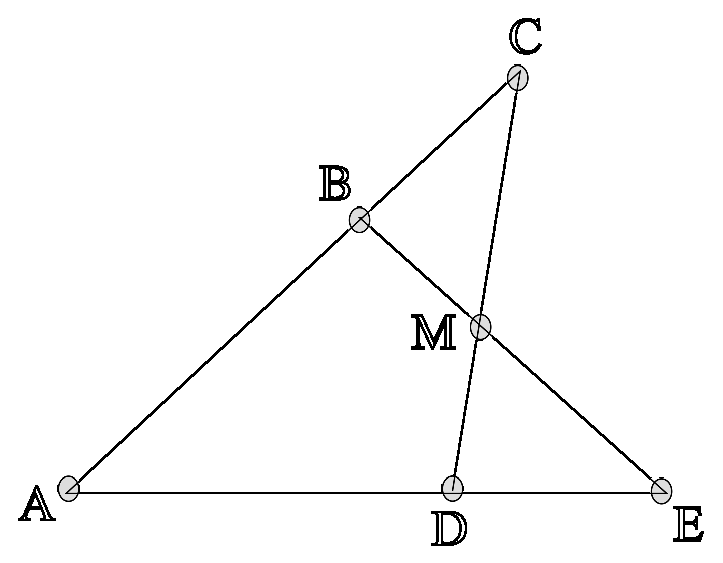
\includegraphics[width=50mm]{problem.eps} \\
\end{tabular}
\end{center}
\answerspacetop

Assume $\overline{BE}$ and $\overline{CD}$ do not intersect, then $\overline{BE} \parallel \overline{CD}$.

That way, $\angle ABE = \angle ACD$; $\angle ADC = \angle AEB$

Also, $\triangle ABE$ and $\triangle ACD$ share $\angle A$

$\therefore \triangle ABE \sim \triangle ACD$

$\because\overline{BE} \parallel \overline{CD}$

$\therefore AB < AC$, $AE < AD$

That contradicts with the fact that $D$ is between $A, E$.\\

This answer is a result of collaboration between Dingwen Wang (UID: 117484526) and Yuchen Liu (UID: 117186154).

\pagebreak


\begin{problem}
Prove that a line cannot be contained in the interior of a triangle.
\end{problem}

\answerspacetop

For line $L$ to be entirely within the interior of $\triangle ABC$, every point on $L$ must lie within the bounded region defined by the sides of $\triangle ABC$, not touching or crossing these sides.

Assume the line $L$ is completely contained in the interior of a $\triangle ABC$.

Since a line extends infinitely in both directions and triangle is a closed shape, it must intersect at least two sides of the $\triangle ABC$. 

But if $L$ intersect with two sides of the $\triangle ABC$, there are at least two points on $L$ that are not in the interior of $\triangle ABC$ but rather on its boundary. This contradicts the assumption that line $L$ is completely contained within the interior of $\triangle ABC$, as having points on the boundary means the line is not entirely in the interior.\\

This answer is a result of collaboration between Dingwen Wang (UID: 117484526) and Yuchen Liu (UID: 117186154).

\pagebreak

\begin{problem}
    A set of points $S$ is called convex if whenever two points $A$ and $B$ are in $S,$
the entire segment $AB$ is contained in $S$. Prove that a half-plane, the
interior of an angle, and the interior of a triangle are all convex sets,
whereas the exterior of a triangle is not convex. Is a triangle a convex set?
\end{problem}

\answerspacetop

\subsection*{Half-Plane}

\textbf{Proof}: Let $H$ be a half-plane, and $L$ be the boundary. Consider $A, B \in H$ and $C$ is a point between $A$ and $B$. If $C \notin H$ then $C$ lies on the another side of the half-plane. Thus $AC$ intersects $L$ at point $T$ and $A$, $C$, $T$ are collinear. We know that $A$, $C$, $B$ are collinear, thus $A$, $T$, $B$ are collinear by the betweenness principle. This implies that $A$ and $B$ are on opposite sides of the plane, not both in set $H$, which is a contradiction.

\subsection*{Intersection of Convex Sets is Convex}

The intersection of any collection of convex sets is convex.

\textbf{Proof}: Let $\{S_i\}$ be a collection of convex sets, and let $S = \bigcap S_i$ be their intersection. We need to show that for any two points $A, B \in S$, the line segment $\overline{AB}$ is entirely contained in $S$.

Since $A, B \in S$, by definition of intersection, $A, B \in S_i$ for all $i$. Given that each $S_i$ is convex, the line segment $\overline{AB}$ is contained in $S_i$ for all $i$. Therefore, $\overline{AB}$ is contained in the intersection $S = \bigcap S_i$, proving that $S$ is convex.

\subsection*{Interior of an Angle}

\textbf{Proof}: The interior of an angle is the intersection of two half-planes $H_1$ and $H_2$. Let's denote the interior of the angle as $S = H_1 \cap H_2$. For any two points $A, B \in S$, they must also lie within both $H_1$ and $H_2$. Since $H_1$ and $H_2$ are convex, the segment $\overline{AB}$ is contained within both $H_1$ and $H_2$, and hence within their intersection $S$. This demonstrates that $S$, the interior of an angle, is convex.

\subsection*{Interior of a Triangle}

\textbf{Proof}: The interior of a triangle is the intersection of three half-planes $H_1$, $H_2$, and $H_3$, each defined by one side of the triangle and containing the triangle. Denote the interior of the triangle as $T = H_1 \cap H_2 \cap H_3$. For any two points $A, B \in T$, since they are within $T$, they lie within each half-plane $H_1$, $H_2$, and $H_3$. Because these half-planes are convex, the segment $\overline{AB}$ lies entirely within each half-plane, and therefore within $T$. This proves that the interior of a triangle is convex.

\subsection*{Exterior of a Triangle}

\textbf{Explanation}: The exterior of a triangle is not convex because there exist two points outside the triangle such that the line segment connecting them passes through the interior of the triangle. This violates the definition of convexity.

\subsection*{Convexity of a Triangle}

\textbf{Explanation}: A triangle is a convex set. This is because, for any two points inside or on the boundary of the triangle, the line segment connecting these points lies entirely within the triangle, satisfying the definition of a convex set.

\pagebreak

\begin{problem}
  Argue from Hilbert's axioms that an arc of a circle contains at least three non-collinear points.
\end{problem}

\answerspacetop
\textbf{Incidence Axioms}
\begin{itemize}
	\item \textbf{Existence of Points on Lines:} For any two points, there exists a line that contains both.
	\item \textbf{Existence of Points on Planes:} For any three points not on the same line, there exists a plane that contains all three.
	\item \textbf{Line Containment:} If two points of a line lie in a plane, then the entire line lies in the plane.
\end{itemize}

\textbf{Order Axioms}
\begin{itemize}
	\item \textbf{Line Betweenness:} If a point $B$ lies between a point $A$ and a point $C$, $A$, $B$, and $C$ are three distinct points of a line, and $B$ lies on the segment $AC$.
	\item \textbf{Segment Construction:} For any line segment, a segment can be extended.
	\item \textbf{Non-collinear:} There exist at least three points not lying on the same line.
\end{itemize}


1. \textbf{Existence of a Circle:} By the axioms of incidence, we know we can have a plane in which a circle is defined.

2. \textbf{Non-collinear Points:} By Non-collinear, we establish the existence of at least three points not lying on the same line. While this axiom directly doesn't address circular arcs, it establishes the principle that not all points must be collinear in a geometric space.

3. \textbf{Three Points on an Arc:} Two points on a circle ($A$ and $B$). By Points on Lines, there exists a line connecting these two points. Since a circle is not a straight line, any segment of the arc cannot be a straight line by the definition of a circle. Now, choose a point $C$ on the arc that is not coincident with the endpoints $A$ and $B$. This point $C$ cannot be collinear with $A$ and $B$ because the shortest distance between two points in a circle is the straight line that connects them. The arc $AB$ demonstrates that these three points are not collinear, as they do not all lie on the straight line segment that would connect $A$ and $B$ directly.

4. \textbf{Using the Circle's Properties:} The fundamental property of a circle (all points equidistant from a center point) ensures that as soon as you have an arc, any three points you pick on that arc will not be collinear. The curvature of the arc guarantees this non-collinearity.\\

This answer is a result of collaboration between Dingwen Wang (UID: 117484526) and Yuchen Liu (UID: 117186154).
\pagebreak

\begin{problem}
    Let $ABCD$ be a quadrilateral such that $m(\angle BAD) = 90^\circ$. Assume $AC = 5$, $BC = 4$, and $DC = 3$. Compute the area of $ABCD$.
\end{problem}
\textit{Hint:} Use coordinates as suggested in the following picture:
\begin{center}
\begin{tabular}{c}
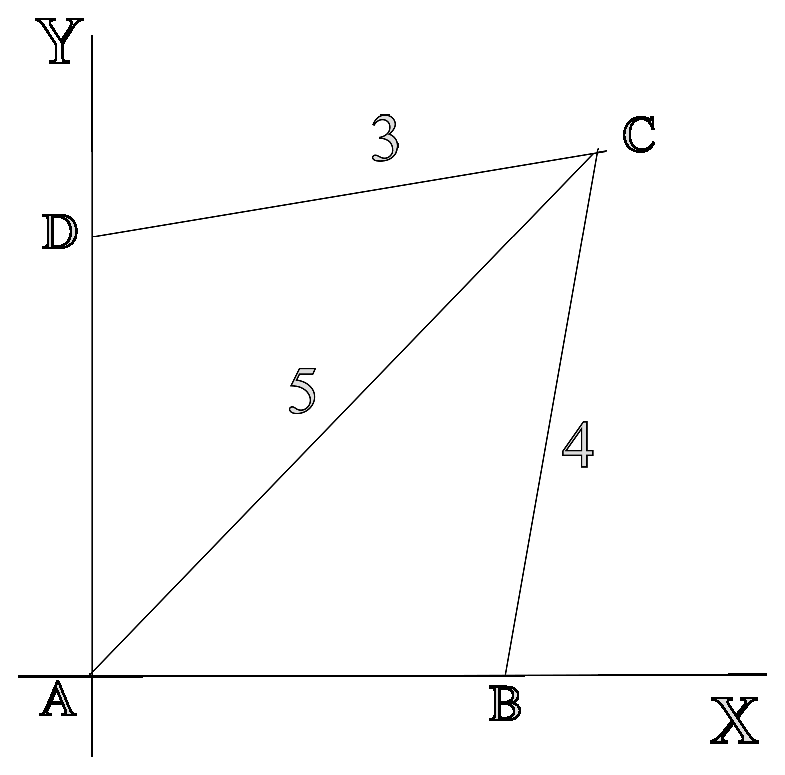
\includegraphics[width=50mm]{problems1.eps} \\
\end{tabular}
\end{center}

\answerspacetop

Take perpendicular line of $X-axis$ cross point $C$, intersect $X-axis$ on point $E$.
Take perpendicular line of $Y-axis$ cross point $C$, intersect $X-axis$ on point $F$.

let $AB = a$
let $AD = b$
let $BE = c$
let $DF = d$

\begin{center}
	\begin{tabular}{c}
		\includegraphics[width=0.5\columnwidth]{Q6.png} \\
	\end{tabular}
\end{center}

From our assumption, $\angle AFC$ and $\angle AEC$ are $90^o$, and we know that $\angle FAE$ is $90^o$ and $AECF$ is a quadrilateral.
Thus $AECF$ is a rectangle, $EC = AF$, $FC = AE$.

$\because$ right $\triangle AEC$ and $\triangle AFC$

$\therefore (a+c)^2 + (b+d)^2 = 5^2$ 

$\therefore a^2 + 2ac + c^2 + b^2 + 2bd + d^2 = 5^2$

$\because$ $\triangle BEC$ and $\triangle DFC$

$\therefore c^2 + EC^2 = 4^2$, $d^2 + FC^2 = 3^2$

$\because 5^2 = 3^2 + 4^2$.

$\therefore a^2 + 2ac + c^2 + b^2 + 2bd + d^2 = c^2 + EC^2 + d^2 + FC^2$

remove $c^2$ and $d^2$, we get $a^2 + 2ac + b^2 + 2bd = EC^2 + FC^2$

Plug-in $EC = b + d$ and $FC = a + c$, we get $a^2 + 2ac + b^2 + 2bd = b^2 + 2bd + d^2 + a^2 + 2ac + c^2$

remove $a^2 + 2ac$ and $b^2 + 2bd$, we get $0 = d^2 + c^2$

$\therefore$ $c = 0$ and $d = 0$, which means $BC$ perpendicular to $X-axis$ and $DC$ perpendicular to Y-axis.

$\therefore$ $ABCD$ is a rectangle with sides 3 and 4.

$Area(ABCD) = 3 * 4 = 12$\\

This answer is a result of collaboration between Dingwen Wang (UID: 117484526) and Yuchen Liu (UID: 117186154).

\pagebreak

\end{document} 